\documentclass[a4paper]{article}
\usepackage{listings}
\usepackage{geometry}
\usepackage{graphicx}
\usepackage{longtable}
\usepackage[colorlinks=true,linkcolor=blue,urlcolor=blue,citecolor=blue]{hyperref}
\usepackage{verbatim}
\usepackage{fancyhdr}
\usepackage{svg}
\svgpath{{figures/}}
\pagestyle{fancy}
\fancyhf{}
\renewcommand{\headrulewidth}{1pt}
\renewcommand{\footrulewidth}{1pt}

\setlength{\headheight}{29.37688pt}

\fancyhead[L]{\includesvg[inkscapelatex=false,width=3cm]{../../logo/logo_forcolormap-roma_8.svg}}
\fancyhead[C]{
	\centering
	\textbf{\LARGE ForColormap}\\
	\textit{Explore the world of colors}
}
\fancyhead[R]{
	\flushright
	\footnotesize{}
}

\fancyfoot[L]{\small \href{https://github.com/vmagnin/forcolormap}{github.com/vmagnin/forcolormap}}
\fancyfoot[C]{\thepage}
\fancyfoot[R]{\small Last updated: \today}

\lstdefinestyle{fortran}{
	language=Fortran,
	basicstyle=\ttfamily,
	keywordstyle=\color{blue},
	commentstyle=\color{green!50!black},
	numbers=left,
	numberstyle=\tiny,
	numbersep=5pt,
	showstringspaces=false,
	breaklines=true,
	frame=single,
	backgroundcolor=\color{gray!10},
	tabsize=4,
	captionpos=b
}


\begin{document}
\begin{titlepage}
	\centering
	\includesvg[inkscapelatex=false,width=8cm]{../../logo/logo_forcolormap-roma_8.svg}\\
	\vspace{1cm}
	{\scshape\LARGE ForColormap}\\
	\vspace{1.5cm}
	{\scshape\Large Explore the world of colors}\\
	\vfill
	{\large \today}\\
\end{titlepage}
\newpage
\tableofcontents
\listoftables
\newpage
\section{Citing Colormaps}
ForColormap includes 222 colormaps from the Scientific coloor maps collection v8.0.1, developed by Fabio Crameri\cite{crameri_2023_8409685}. The colormaps acton*, bam*, bamako*, batlow*, berlin*, bilbao*, broc*, buda*, bukavu*, cork*, davos*, devon*, fes*, glasgow*, grayc*, hawaii*, imola*, lajolla*, lapaz*, lipari*, lisbon*, managua*, navia*, nuuk*, oleron*, oslo*, roma*, tofino*, tokyo*, turku*, vanimo*, and vik*, are part of the Scientific Colormap Collection. If you use any of these colormaps, please cite this paper \cite{Crameri2020}. Additionally, the colormaps magma, inferno, plasma, and viridis are sourced from the matplotlib colormaps. When employing these colormaps, please cite this webpage\cite{mpl_colormaps}. For the cubehelix colormap, please cite\cite{green2011colour}. For the black\_body colormap, please cite\cite{color_advice}.

\newpage
\section{Basic Usage}
Assuming your graphical library has a \texttt{setpixelgb()}-like function and you know your $z$ values will be for example in the $[0, 2]$ range, you can write something like:
\begin{lstlisting}[style=fortran]
use forcolormap, only: Colormap, colormaps_list, wp
...
type(Colormap) :: cmap
integer  :: red, green, blue
real(wp) :: z, x, y
...
! Let's use the glasgow colormap:
call cmap%set("glasgow", 0.0_wp, 2.0_wp)
...
z = f(x,y)
call cmap%compute_RGB(z, red, green, blue)
call setpixelrgb(x, y, red, green, blue)
\end{lstlisting}
\newpage
\section{Colormaps}
\subsection{Sequential Gradients}
\renewcommand{\arraystretch}{2}
\begin{longtable}{p{0.15\textwidth}p{0.15\textwidth}p{0.1\textwidth}p{0.1\textwidth}p{0.35\textwidth}}
	\caption{Sequential Gradients} \label{tab:seq}                                             \\
	\hline
	\textbf{Name} & \textbf{Gradient} & \textbf{Palette} & \textbf{Levels} & \textbf{Colorbar} \\ \hline \endfirsthead
	\caption*{Table \ref{tab:seq} Continued: Sequential Gradients}                             \\
	\hline
	\textbf{Name} & \textbf{Gradient} & \textbf{Palette} & \textbf{Levels} & \textbf{Colorbar} \\ \hline \endhead
	acton & Sequential & Continuous & 256 &

\includegraphics[width=\linewidth]{../png/acton_colorbar.png}\\ \hline
acton10 & Sequential & Discrete & 10 &

\includegraphics[width=\linewidth]{../png/acton10_colorbar.png}\\ \hline
acton25 & Sequential & Discrete & 25 &

\includegraphics[width=\linewidth]{../png/acton25_colorbar.png}\\ \hline
acton50 & Sequential & Discrete & 50 &

\includegraphics[width=\linewidth]{../png/acton50_colorbar.png}\\ \hline
acton100 & Sequential & Discrete & 100 &

\includegraphics[width=\linewidth]{../png/acton100_colorbar.png}\\ \hline
bamako & Sequential & Continuous & 256 &

\includegraphics[width=\linewidth]{../png/bamako_colorbar.png}\\ \hline
bamako10 & Sequential & Discrete & 10 &

\includegraphics[width=\linewidth]{../png/bamako10_colorbar.png}\\ \hline
bamako100 & Sequential & Discrete & 100 &

\includegraphics[width=\linewidth]{../png/bamako100_colorbar.png}\\ \hline
bamako25 & Sequential & Discrete & 25 &

\includegraphics[width=\linewidth]{../png/bamako25_colorbar.png}\\ \hline
bamako50 & Sequential & Discrete & 50 &

\includegraphics[width=\linewidth]{../png/bamako50_colorbar.png}\\ \hline
batlow & Sequential & Continuous & 256 &

\includegraphics[width=\linewidth]{../png/batlow_colorbar.png}\\ \hline
batlow10 & Sequential & Discrete & 10 &

\includegraphics[width=\linewidth]{../png/batlow10_colorbar.png}\\ \hline
batlow100 & Sequential & Discrete & 100 &

\includegraphics[width=\linewidth]{../png/batlow100_colorbar.png}\\ \hline
batlow25 & Sequential & Discrete & 25 &

\includegraphics[width=\linewidth]{../png/batlow25_colorbar.png}\\ \hline
batlow50 & Sequential & Discrete & 50 &

\includegraphics[width=\linewidth]{../png/batlow50_colorbar.png}\\ \hline
batlowK & Sequential & Continuous & 256 &
\includegraphics[width=\linewidth]{../png/batlowk_colorbar.png}\\ \hline
batlowK10 & Sequential & Discrete & 10 &
\includegraphics[width=\linewidth]{../png/batlowk10_colorbar.png}\\ \hline
batlowK100 & Sequential & Discrete & 100 &
\includegraphics[width=\linewidth]{../png/batlowk100_colorbar.png}\\ \hline
batlowK25 & Sequential & Discrete & 25 &
\includegraphics[width=\linewidth]{../png/batlowk25_colorbar.png}\\ \hline
batlowK50 & Sequential & Discrete & 50 &
\includegraphics[width=\linewidth]{../png/batlowk50_colorbar.png}\\ \hline
batlowW & Sequential & Continuous & 256 &
\includegraphics[width=\linewidth]{../png/batloww_colorbar.png}\\ \hline
batlowW10 & Sequential & Discrete & 10 &
\includegraphics[width=\linewidth]{../png/batloww10_colorbar.png}\\ \hline
batlowW100 & Sequential & Discrete & 100 &
\includegraphics[width=\linewidth]{../png/batloww100_colorbar.png}\\ \hline
batlowW25 & Sequential & Discrete & 25 &
\includegraphics[width=\linewidth]{../png/batloww25_colorbar.png}\\ \hline
batlowW50 & Sequential & Discrete & 50 &
\includegraphics[width=\linewidth]{../png/batloww50_colorbar.png}\\ \hline
bilbao & Sequential & Continuous & 256 &

\includegraphics[width=\linewidth]{../png/bilbao_colorbar.png}\\ \hline
bilbao10 & Sequential & Discrete & 10 &

\includegraphics[width=\linewidth]{../png/bilbao10_colorbar.png}\\ \hline
bilbao100 & Sequential & Discrete & 100 &

\includegraphics[width=\linewidth]{../png/bilbao100_colorbar.png}\\ \hline
bilbao25 & Sequential & Discrete & 25 &

\includegraphics[width=\linewidth]{../png/bilbao25_colorbar.png}\\ \hline
bilbao50 & Sequential & Discrete & 50 &

\includegraphics[width=\linewidth]{../png/bilbao50_colorbar.png}\\ \hline
buda & Sequential & Continuous & 256 &

\includegraphics[width=\linewidth]{../png/buda_colorbar.png}\\ \hline
buda10 & Sequential & Discrete & 10 &

\includegraphics[width=\linewidth]{../png/buda10_colorbar.png}\\ \hline
buda100 & Sequential & Discrete & 100 &

\includegraphics[width=\linewidth]{../png/buda100_colorbar.png}\\ \hline
buda25 & Sequential & Discrete & 25 &
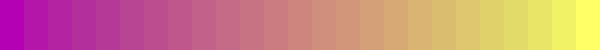
\includegraphics[width=\linewidth]{../png/buda25_colorbar.png}\\ \hline
buda50 & Sequential & Discrete & 50 &

\includegraphics[width=\linewidth]{../png/buda50_colorbar.png}\\ \hline
davos & Sequential & Continuous & 256 &

\includegraphics[width=\linewidth]{../png/davos_colorbar.png}\\ \hline
davos10 & Sequential & Discrete & 10 &

\includegraphics[width=\linewidth]{../png/davos10_colorbar.png}\\ \hline
davos100 & Sequential & Discrete & 100 &

\includegraphics[width=\linewidth]{../png/davos100_colorbar.png}\\ \hline
davos25 & Sequential & Discrete & 25 &

\includegraphics[width=\linewidth]{../png/davos25_colorbar.png}\\ \hline
davos50 & Sequential & Discrete & 50 &

\includegraphics[width=\linewidth]{../png/davos50_colorbar.png}\\ \hline
devon & Sequential & Continuous & 256 &

\includegraphics[width=\linewidth]{../png/devon_colorbar.png}\\ \hline
devon10 & Sequential & Discrete & 10 &

\includegraphics[width=\linewidth]{../png/devon10_colorbar.png}\\ \hline
devon100 & Sequential & Discrete & 100 &

\includegraphics[width=\linewidth]{../png/devon100_colorbar.png}\\ \hline
devon25 & Sequential & Discrete & 25 &

\includegraphics[width=\linewidth]{../png/devon25_colorbar.png}\\ \hline
devon50 & Sequential & Discrete & 50 &

\includegraphics[width=\linewidth]{../png/devon50_colorbar.png}\\ \hline
glasgow & Sequential & Continuous & 256 &

\includegraphics[width=\linewidth]{../png/glasgow_colorbar.png}\\ \hline
glasgow10 & Sequential & Discrete & 10 &

\includegraphics[width=\linewidth]{../png/glasgow10_colorbar.png}\\ \hline
glasgow100 & Sequential & Discrete & 100 &

\includegraphics[width=\linewidth]{../png/glasgow100_colorbar.png}\\ \hline
glasgow25 & Sequential & Discrete & 25 &
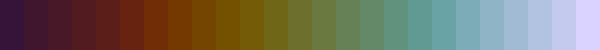
\includegraphics[width=\linewidth]{../png/glasgow25_colorbar.png}\\ \hline
glasgow50 & Sequential & Discrete & 50 &

\includegraphics[width=\linewidth]{../png/glasgow50_colorbar.png}\\ \hline
grayC & Sequential & Continuous & 256 &
\includegraphics[width=\linewidth]{../png/grayc_colorbar.png}\\ \hline
grayC10 & Sequential & Discrete & 10 &
\includegraphics[width=\linewidth]{../png/grayc10_colorbar.png}\\ \hline
grayC100 & Sequential & Discrete & 100 &
\includegraphics[width=\linewidth]{../png/grayc100_colorbar.png}\\ \hline
grayC25 & Sequential & Discrete & 25 &
\includegraphics[width=\linewidth]{../png/grayc25_colorbar.png}\\ \hline
grayC50 & Sequential & Discrete & 50 &
\includegraphics[width=\linewidth]{../png/grayc50_colorbar.png}\\ \hline
hawaii & Sequential & Continuous & 256 &
\includegraphics[width=\linewidth]{../png/hawaii_colorbar.png}\\ \hline
hawaii10 & Sequential & Discrete & 10 &
\includegraphics[width=\linewidth]{../png/hawaii10_colorbar.png}\\ \hline
hawaii100 & Sequential & Discrete & 100 &
\includegraphics[width=\linewidth]{../png/hawaii100_colorbar.png}\\ \hline
hawaii25 & Sequential & Discrete & 25 &
\includegraphics[width=\linewidth]{../png/hawaii25_colorbar.png}\\ \hline
hawaii50 & Sequential & Discrete & 50 &
\includegraphics[width=\linewidth]{../png/hawaii50_colorbar.png}\\ \hline
imola & Sequential & Continuous & 256 &
\includegraphics[width=\linewidth]{../png/imola_colorbar.png}\\ \hline
imola10 & Sequential & Discrete & 10 &
\includegraphics[width=\linewidth]{../png/imola10_colorbar.png}\\ \hline
imola100 & Sequential & Discrete & 100 &
\includegraphics[width=\linewidth]{../png/imola100_colorbar.png}\\ \hline
imola25 & Sequential & Discrete & 25 &
\includegraphics[width=\linewidth]{../png/imola25_colorbar.png}\\ \hline
imola50 & Sequential & Discrete & 50 &
\includegraphics[width=\linewidth]{../png/imola50_colorbar.png}\\ \hline
lajolla & Sequential & Continuous & 256 &
\includegraphics[width=\linewidth]{../png/lajolla_colorbar.png}\\ \hline
lajolla10 & Sequential & Discrete & 10 &
\includegraphics[width=\linewidth]{../png/lajolla10_colorbar.png}\\ \hline
lajolla100 & Sequential & Discrete & 100 &
\includegraphics[width=\linewidth]{../png/lajolla100_colorbar.png}\\ \hline
lajolla25 & Sequential & Discrete & 25 &
\includegraphics[width=\linewidth]{../png/lajolla25_colorbar.png}\\ \hline
lajolla50 & Sequential & Discrete & 50 &
\includegraphics[width=\linewidth]{../png/lajolla50_colorbar.png}\\ \hline
lapaz & Sequential & Continuous & 256 &
\includegraphics[width=\linewidth]{../png/lapaz_colorbar.png}\\ \hline
lapaz10 & Sequential & Discrete & 10 &
\includegraphics[width=\linewidth]{../png/lapaz10_colorbar.png}\\ \hline
lapaz100 & Sequential & Discrete & 100 &
\includegraphics[width=\linewidth]{../png/lapaz100_colorbar.png}\\ \hline
lapaz25 & Sequential & Discrete & 25 &
\includegraphics[width=\linewidth]{../png/lapaz25_colorbar.png}\\ \hline
lapaz50 & Sequential & Discrete & 50 &
\includegraphics[width=\linewidth]{../png/lapaz50_colorbar.png}\\ \hline
lipari & Sequential & Continuous & 256 &
\includegraphics[width=\linewidth]{../png/lipari_colorbar.png}\\ \hline
lipari10 & Sequential & Discrete & 10 &
\includegraphics[width=\linewidth]{../png/lipari10_colorbar.png}\\ \hline
lipari100 & Sequential & Discrete & 100 &
\includegraphics[width=\linewidth]{../png/lipari100_colorbar.png}\\ \hline
lipari25 & Sequential & Discrete & 25 &
\includegraphics[width=\linewidth]{../png/lipari25_colorbar.png}\\ \hline
lipari50 & Sequential & Discrete & 50 &
\includegraphics[width=\linewidth]{../png/lipari50_colorbar.png}\\ \hline
navia & Sequential & Continuous & 256 &
\includegraphics[width=\linewidth]{../png/navia_colorbar.png}\\ \hline
navia10 & Sequential & Discrete & 10 &
\includegraphics[width=\linewidth]{../png/navia10_colorbar.png}\\ \hline
navia100 & Sequential & Discrete & 100 &
\includegraphics[width=\linewidth]{../png/navia100_colorbar.png}\\ \hline
navia25 & Sequential & Discrete & 25 &
\includegraphics[width=\linewidth]{../png/navia25_colorbar.png}\\ \hline
navia50 & Sequential & Discrete & 50 &
\includegraphics[width=\linewidth]{../png/navia50_colorbar.png}\\ \hline
naviaW & Sequential & Continuous & 256 &
\includegraphics[width=\linewidth]{../png/naviaw_colorbar.png}\\ \hline
naviaW10 & Sequential & Discrete & 10 &
\includegraphics[width=\linewidth]{../png/naviaw10_colorbar.png}\\ \hline
naviaW100 & Sequential & Discrete & 100 &
\includegraphics[width=\linewidth]{../png/naviaw100_colorbar.png}\\ \hline
naviaW25 & Sequential & Discrete & 25 &
\includegraphics[width=\linewidth]{../png/naviaw25_colorbar.png}\\ \hline
naviaW50 & Sequential & Discrete & 50 &
\includegraphics[width=\linewidth]{../png/naviaw50_colorbar.png}\\ \hline
nuuk & Sequential & Continuous & 256 &
\includegraphics[width=\linewidth]{../png/nuuk_colorbar.png}\\ \hline
nuuk10 & Sequential & Discrete & 10 &
\includegraphics[width=\linewidth]{../png/nuuk10_colorbar.png}\\ \hline
nuuk100 & Sequential & Discrete & 100 &
\includegraphics[width=\linewidth]{../png/nuuk100_colorbar.png}\\ \hline
nuuk25 & Sequential & Discrete & 25 &
\includegraphics[width=\linewidth]{../png/nuuk25_colorbar.png}\\ \hline
nuuk50 & Sequential & Discrete & 50 &
\includegraphics[width=\linewidth]{../png/nuuk50_colorbar.png}\\ \hline
oslo & Sequential & Continuous & 256 &
\includegraphics[width=\linewidth]{../png/oslo_colorbar.png}\\ \hline
oslo10 & Sequential & Discrete & 10 &
\includegraphics[width=\linewidth]{../png/oslo10_colorbar.png}\\ \hline
oslo100 & Sequential & Discrete & 100 &
\includegraphics[width=\linewidth]{../png/oslo100_colorbar.png}\\ \hline
oslo25 & Sequential & Discrete & 25 &
\includegraphics[width=\linewidth]{../png/oslo25_colorbar.png}\\ \hline
oslo50 & Sequential & Discrete & 50 &
\includegraphics[width=\linewidth]{../png/oslo50_colorbar.png}\\ \hline
tokyo & Sequential & Continuous & 256 &
\includegraphics[width=\linewidth]{../png/tokyo_colorbar.png}\\ \hline
tokyo10 & Sequential & Discrete & 10 &
\includegraphics[width=\linewidth]{../png/tokyo10_colorbar.png}\\ \hline
tokyo100 & Sequential & Discrete & 100 &
\includegraphics[width=\linewidth]{../png/tokyo100_colorbar.png}\\ \hline
tokyo25 & Sequential & Discrete & 25 &
\includegraphics[width=\linewidth]{../png/tokyo25_colorbar.png}\\ \hline
tokyo50 & Sequential & Discrete & 50 &
\includegraphics[width=\linewidth]{../png/tokyo50_colorbar.png}\\ \hline
turku & Sequential & Continuous & 256 &
\includegraphics[width=\linewidth]{../png/turku_colorbar.png}\\ \hline
turku10 & Sequential & Discrete & 10 &
\includegraphics[width=\linewidth]{../png/turku10_colorbar.png}\\ \hline
turku100 & Sequential & Discrete & 100 &
\includegraphics[width=\linewidth]{../png/turku100_colorbar.png}\\ \hline
turku25 & Sequential & Discrete & 25 &
\includegraphics[width=\linewidth]{../png/turku25_colorbar.png}\\ \hline
turku50 & Sequential & Discrete & 50 &
\includegraphics[width=\linewidth]{../png/turku50_colorbar.png}\\ \hline
black\_body & Sequential & Continuous & 1024 &
\includegraphics[width=\linewidth]{../png/black_body_colorbar.png}\\ \hline
fire & Sequential & Continuous & -1 &
\includegraphics[width=\linewidth]{../png/fire_colorbar.png}\\ \hline
cubehelix & Sequential & Continuous & -1 &
\includegraphics[width=\linewidth]{../png/cubehelix_colorbar.png}\\ \hline

\end{longtable}
\newpage
\subsection{Diverging Gradients}
\renewcommand{\arraystretch}{2}
\begin{longtable}{p{0.15\textwidth}p{0.15\textwidth}p{0.1\textwidth}p{0.1\textwidth}p{0.35\textwidth}}
	\caption{Diverging Gradients} \label{tab:div}                                              \\
	\hline
	\textbf{Name} & \textbf{Gradient} & \textbf{Palette} & \textbf{Levels} & \textbf{Colorbar} \\ \hline \endfirsthead
	\caption*{Table \ref{tab:seq} Continued: Diverging Gradients}                              \\
	\hline
	\textbf{Name} & \textbf{Gradient} & \textbf{Palette} & \textbf{Levels} & \textbf{Colorbar} \\ \hline \endhead
	bam & Diverging & Continuous & 256 &
\includegraphics[width=\linewidth]{../png/bam_colorbar.png}\\ \hline
bam10 & Diverging & Discrete & 10 &
\includegraphics[width=\linewidth]{../png/bam10_colorbar.png}\\ \hline
bam100 & Diverging & Discrete & 100 &
\includegraphics[width=\linewidth]{../png/bam100_colorbar.png}\\ \hline
bam25 & Diverging & Discrete & 25 &
\includegraphics[width=\linewidth]{../png/bam25_colorbar.png}\\ \hline
bam50 & Diverging & Discrete & 50 &
\includegraphics[width=\linewidth]{../png/bam50_colorbar.png}\\ \hline
berlin & Diverging & Continuous & 256 &
\includegraphics[width=\linewidth]{../png/berlin_colorbar.png}\\ \hline
berlin10 & Diverging & Discrete & 10 &
\includegraphics[width=\linewidth]{../png/berlin10_colorbar.png}\\ \hline
berlin100 & Diverging & Discrete & 100 &
\includegraphics[width=\linewidth]{../png/berlin100_colorbar.png}\\ \hline
berlin25 & Diverging & Discrete & 25 &
\includegraphics[width=\linewidth]{../png/berlin25_colorbar.png}\\ \hline
berlin50 & Diverging & Discrete & 50 &
\includegraphics[width=\linewidth]{../png/berlin50_colorbar.png}\\ \hline
broc & Diverging & Continuous & 256 &
\includegraphics[width=\linewidth]{../png/broc_colorbar.png}\\ \hline
broc10 & Diverging & Discrete & 10 &
\includegraphics[width=\linewidth]{../png/broc10_colorbar.png}\\ \hline
broc100 & Diverging & Discrete & 100 &
\includegraphics[width=\linewidth]{../png/broc100_colorbar.png}\\ \hline
broc25 & Diverging & Discrete & 25 &
\includegraphics[width=\linewidth]{../png/broc25_colorbar.png}\\ \hline
broc50 & Diverging & Discrete & 50 &
\includegraphics[width=\linewidth]{../png/broc50_colorbar.png}\\ \hline
brocO10 & Diverging & Discrete & 10 &
\includegraphics[width=\linewidth]{../png/broco10_colorbar.png}\\ \hline
brocO100 & Diverging & Discrete & 100 &
\includegraphics[width=\linewidth]{../png/broco100_colorbar.png}\\ \hline
brocO25 & Diverging & Discrete & 25 &
\includegraphics[width=\linewidth]{../png/broco25_colorbar.png}\\ \hline
brocO50 & Diverging & Discrete & 50 &
\includegraphics[width=\linewidth]{../png/broco50_colorbar.png}\\ \hline
cork & Diverging & Continuous & 256 &
\includegraphics[width=\linewidth]{../png/cork_colorbar.png}\\ \hline
cork10 & Diverging & Discrete & 10 &
\includegraphics[width=\linewidth]{../png/cork10_colorbar.png}\\ \hline
cork100 & Diverging & Discrete & 100 &
\includegraphics[width=\linewidth]{../png/cork100_colorbar.png}\\ \hline
cork25 & Diverging & Discrete & 25 &
\includegraphics[width=\linewidth]{../png/cork25_colorbar.png}\\ \hline
cork50 & Diverging & Discrete & 50 &
\includegraphics[width=\linewidth]{../png/cork50_colorbar.png}\\ \hline
corkO10 & Diverging & Discrete & 10 &
\includegraphics[width=\linewidth]{../png/corko10_colorbar.png}\\ \hline
corkO100 & Diverging & Discrete & 100 &
\includegraphics[width=\linewidth]{../png/corko100_colorbar.png}\\ \hline
corkO25 & Diverging & Discrete & 25 &
\includegraphics[width=\linewidth]{../png/corko25_colorbar.png}\\ \hline
corkO50 & Diverging & Discrete & 50 &
\includegraphics[width=\linewidth]{../png/corko50_colorbar.png}\\ \hline
lisbon & Diverging & Continuous & 256 &
\includegraphics[width=\linewidth]{../png/lisbon_colorbar.png}\\ \hline
lisbon10 & Diverging & Discrete & 10 &
\includegraphics[width=\linewidth]{../png/lisbon10_colorbar.png}\\ \hline
lisbon100 & Diverging & Discrete & 100 &
\includegraphics[width=\linewidth]{../png/lisbon100_colorbar.png}\\ \hline
lisbon25 & Diverging & Discrete & 25 &
\includegraphics[width=\linewidth]{../png/lisbon25_colorbar.png}\\ \hline
lisbon50 & Diverging & Discrete & 50 &
\includegraphics[width=\linewidth]{../png/lisbon50_colorbar.png}\\ \hline
managua & Diverging & Continuous & 256 &
\includegraphics[width=\linewidth]{../png/managua_colorbar.png}\\ \hline
managua10 & Diverging & Discrete & 10 &
\includegraphics[width=\linewidth]{../png/managua10_colorbar.png}\\ \hline
managua100 & Diverging & Discrete & 100 &
\includegraphics[width=\linewidth]{../png/managua100_colorbar.png}\\ \hline
managua25 & Diverging & Discrete & 25 &
\includegraphics[width=\linewidth]{../png/managua25_colorbar.png}\\ \hline
managua50 & Diverging & Discrete & 50 &
\includegraphics[width=\linewidth]{../png/managua50_colorbar.png}\\ \hline
roma & Diverging & Continuous & 256 &
\includegraphics[width=\linewidth]{../png/roma_colorbar.png}\\ \hline
roma10 & Diverging & Discrete & 10 &
\includegraphics[width=\linewidth]{../png/roma10_colorbar.png}\\ \hline
roma100 & Diverging & Discrete & 100 &
\includegraphics[width=\linewidth]{../png/roma100_colorbar.png}\\ \hline
roma25 & Diverging & Discrete & 25 &
\includegraphics[width=\linewidth]{../png/roma25_colorbar.png}\\ \hline
roma50 & Diverging & Discrete & 50 &
\includegraphics[width=\linewidth]{../png/roma50_colorbar.png}\\ \hline
romaO10 & Diverging & Discrete & 10 &
\includegraphics[width=\linewidth]{../png/romao10_colorbar.png}\\ \hline
romaO100 & Diverging & Discrete & 100 &
\includegraphics[width=\linewidth]{../png/romao100_colorbar.png}\\ \hline
romaO25 & Diverging & Discrete & 25 &
\includegraphics[width=\linewidth]{../png/romao25_colorbar.png}\\ \hline
romaO50 & Diverging & Discrete & 50 &
\includegraphics[width=\linewidth]{../png/romao50_colorbar.png}\\ \hline
tofino & Diverging & Continuous & 256 &
\includegraphics[width=\linewidth]{../png/tofino_colorbar.png}\\ \hline
tofino10 & Diverging & Discrete & 10 &
\includegraphics[width=\linewidth]{../png/tofino10_colorbar.png}\\ \hline
tofino100 & Diverging & Discrete & 100 &
\includegraphics[width=\linewidth]{../png/tofino100_colorbar.png}\\ \hline
tofino25 & Diverging & Discrete & 25 &
\includegraphics[width=\linewidth]{../png/tofino25_colorbar.png}\\ \hline
tofino50 & Diverging & Discrete & 50 &
\includegraphics[width=\linewidth]{../png/tofino50_colorbar.png}\\ \hline
vanimo & Diverging & Continuous & 256 &
\includegraphics[width=\linewidth]{../png/vanimo_colorbar.png}\\ \hline
vanimo10 & Diverging & Discrete & 10 &
\includegraphics[width=\linewidth]{../png/vanimo10_colorbar.png}\\ \hline
vanimo100 & Diverging & Discrete & 100 &
\includegraphics[width=\linewidth]{../png/vanimo100_colorbar.png}\\ \hline
vanimo25 & Diverging & Discrete & 25 &
\includegraphics[width=\linewidth]{../png/vanimo25_colorbar.png}\\ \hline
vanimo50 & Diverging & Discrete & 50 &
\includegraphics[width=\linewidth]{../png/vanimo50_colorbar.png}\\ \hline
vik & Diverging & Continuous & 256 &
\includegraphics[width=\linewidth]{../png/vik_colorbar.png}\\ \hline
vik10 & Diverging & Discrete & 10 &
\includegraphics[width=\linewidth]{../png/vik10_colorbar.png}\\ \hline
vik100 & Diverging & Discrete & 100 &
\includegraphics[width=\linewidth]{../png/vik100_colorbar.png}\\ \hline
vik25 & Diverging & Discrete & 25 &
\includegraphics[width=\linewidth]{../png/vik25_colorbar.png}\\ \hline
vik50 & Diverging & Discrete & 50 &
\includegraphics[width=\linewidth]{../png/vik50_colorbar.png}\\ \hline
vikO10 & Diverging & Discrete & 10 &
\includegraphics[width=\linewidth]{../png/viko10_colorbar.png}\\ \hline
vikO100 & Diverging & Discrete & 100 &
\includegraphics[width=\linewidth]{../png/viko100_colorbar.png}\\ \hline
vikO25 & Diverging & Discrete & 25 &
\includegraphics[width=\linewidth]{../png/viko25_colorbar.png}\\ \hline
vikO50 & Diverging & Discrete & 50 &
\includegraphics[width=\linewidth]{../png/viko50_colorbar.png}\\ \hline

\end{longtable}
\newpage
\subsection{Cyclic Gradients}
\renewcommand{\arraystretch}{2}
\begin{longtable}{p{0.15\textwidth}p{0.15\textwidth}p{0.1\textwidth}p{0.1\textwidth}p{0.35\textwidth}}
	\caption{Cyclic Gradients} \label{tab:cyc}                                                 \\
	\hline
	\textbf{Name} & \textbf{Gradient} & \textbf{Palette} & \textbf{Levels} & \textbf{Colorbar} \\ \hline \endfirsthead
	\caption*{Table \ref{tab:seq} Continued: Cyclic Gradients}                                 \\
	\hline
	\textbf{Name} & \textbf{Gradient} & \textbf{Palette} & \textbf{Levels} & \textbf{Colorbar} \\ \hline \endhead
	bamO & Cyclic & Continuous & 256 &
\includegraphics[width=\linewidth]{../png/bamo_colorbar.png}\\ \hline
bamO10 & Cyclic & Discrete & 10 &
\includegraphics[width=\linewidth]{../png/bamo10_colorbar.png}\\ \hline
bamO100 & Cyclic & Discrete & 100 &
\includegraphics[width=\linewidth]{../png/bamo100_colorbar.png}\\ \hline
bamO25 & Cyclic & Discrete & 25 &
\includegraphics[width=\linewidth]{../png/bamo25_colorbar.png}\\ \hline
bamO50 & Cyclic & Discrete & 50 &
\includegraphics[width=\linewidth]{../png/bamo50_colorbar.png}\\ \hline
brocO & Cyclic & Continuous & 256 &
\includegraphics[width=\linewidth]{../png/broco_colorbar.png}\\ \hline
corkO & Cyclic & Continuous & 256 &
\includegraphics[width=\linewidth]{../png/corko_colorbar.png}\\ \hline
romaO & Cyclic & Continuous & 256 &
\includegraphics[width=\linewidth]{../png/romao_colorbar.png}\\ \hline
vikO & Cyclic & Continuous & 256 &
\includegraphics[width=\linewidth]{../png/viko_colorbar.png}\\ \hline

\end{longtable}
\newpage
\subsection{Multi-Sequential Gradients}
\renewcommand{\arraystretch}{2}
\begin{longtable}{p{0.15\textwidth}p{0.15\textwidth}p{0.1\textwidth}p{0.1\textwidth}p{0.35\textwidth}}
	\caption{Multi-Sequential Gradients} \label{tab:msq}                                       \\
	\hline
	\textbf{Name} & \textbf{Gradient} & \textbf{Palette} & \textbf{Levels} & \textbf{Colorbar} \\ \hline \endfirsthead
	\caption*{Table \ref{tab:seq} Continued: Multi Sequential Gradients}                       \\
	\hline
	\textbf{Name} & \textbf{Gradient} & \textbf{Palette} & \textbf{Levels} & \textbf{Colorbar} \\ \hline \endhead
	bukavu & Multi-Sequential & Continuous & 256 &
\includegraphics[width=\linewidth]{../png/bukavu_colorbar.png}\\ \hline
bukavu10 & Multi-Sequential & Discrete & 10 &
\includegraphics[width=\linewidth]{../png/bukavu10_colorbar.png}\\ \hline
bukavu100 & Multi-Sequential & Discrete & 100 &
\includegraphics[width=\linewidth]{../png/bukavu100_colorbar.png}\\ \hline
bukavu25 & Multi-Sequential & Discrete & 25 &
\includegraphics[width=\linewidth]{../png/bukavu25_colorbar.png}\\ \hline
bukavu50 & Multi-Sequential & Discrete & 50 &
\includegraphics[width=\linewidth]{../png/bukavu50_colorbar.png}\\ \hline
fes & Multi-Sequential & Continuous & 256 &
\includegraphics[width=\linewidth]{../png/fes_colorbar.png}\\ \hline
fes10 & Multi-Sequential & Discrete & 10 &
\includegraphics[width=\linewidth]{../png/fes10_colorbar.png}\\ \hline
fes100 & Multi-Sequential & Discrete & 100 &
\includegraphics[width=\linewidth]{../png/fes100_colorbar.png}\\ \hline
fes25 & Multi-Sequential & Discrete & 25 &
\includegraphics[width=\linewidth]{../png/fes25_colorbar.png}\\ \hline
fes50 & Multi-Sequential & Discrete & 50 &
\includegraphics[width=\linewidth]{../png/fes50_colorbar.png}\\ \hline
oleron & Multi-Sequential & Continuous & 256 &
\includegraphics[width=\linewidth]{../png/oleron_colorbar.png}\\ \hline
oleron10 & Multi-Sequential & Discrete & 10 &
\includegraphics[width=\linewidth]{../png/oleron10_colorbar.png}\\ \hline
oleron100 & Multi-Sequential & Discrete & 100 &
\includegraphics[width=\linewidth]{../png/oleron100_colorbar.png}\\ \hline
oleron25 & Multi-Sequential & Discrete & 25 &
\includegraphics[width=\linewidth]{../png/oleron25_colorbar.png}\\ \hline
oleron50 & Multi-Sequential & Discrete & 50 &
\includegraphics[width=\linewidth]{../png/oleron50_colorbar.png}\\ \hline

\end{longtable}
\newpage
\subsection{Categorical Gradients}
\renewcommand{\arraystretch}{2}
\begin{longtable}{p{0.15\textwidth}p{0.15\textwidth}p{0.1\textwidth}p{0.1\textwidth}p{0.35\textwidth}}
	\caption{Categorical Gradients} \label{tab:cat}                                            \\
	\hline
	\textbf{Name} & \textbf{Gradient} & \textbf{Palette} & \textbf{Levels} & \textbf{Colorbar} \\ \hline \endfirsthead
	\caption*{Table \ref{tab:seq} Continued: Categorical Gradients}                            \\
	\hline
	\textbf{Name} & \textbf{Gradient} & \textbf{Palette} & \textbf{Levels} & \textbf{Colorbar} \\ \hline \endhead
	actonS & Categorical & Continuous & 256 &
\includegraphics[width=\linewidth]{../png/actons_colorbar.png}\\ \hline
bamakoS & Categorical & Continuous & 256 &
\includegraphics[width=\linewidth]{../png/bamakos_colorbar.png}\\ \hline
batlowKS & Categorical & Continuous & 256 &
\includegraphics[width=\linewidth]{../png/batlowks_colorbar.png}\\ \hline
batlowS & Categorical & Continuous & 256 &
\includegraphics[width=\linewidth]{../png/batlows_colorbar.png}\\ \hline
batlowWS & Categorical & Continuous & 256 &
\includegraphics[width=\linewidth]{../png/batlowws_colorbar.png}\\ \hline
bilbaoS & Categorical & Continuous & 256 &
\includegraphics[width=\linewidth]{../png/bilbaos_colorbar.png}\\ \hline
budaS & Categorical & Continuous & 256 &
\includegraphics[width=\linewidth]{../png/budas_colorbar.png}\\ \hline
davosS & Categorical & Continuous & 256 &
\includegraphics[width=\linewidth]{../png/davoss_colorbar.png}\\ \hline
devonS & Categorical & Continuous & 256 &
\includegraphics[width=\linewidth]{../png/devons_colorbar.png}\\ \hline
glasgowS & Categorical & Continuous & 256 &
\includegraphics[width=\linewidth]{../png/glasgows_colorbar.png}\\ \hline
grayCS & Categorical & Continuous & 256 &
\includegraphics[width=\linewidth]{../png/graycs_colorbar.png}\\ \hline
hawaiiS & Categorical & Continuous & 256 &
\includegraphics[width=\linewidth]{../png/hawaiis_colorbar.png}\\ \hline
imolaS & Categorical & Continuous & 256 &
\includegraphics[width=\linewidth]{../png/imolas_colorbar.png}\\ \hline
lajollaS & Categorical & Continuous & 256 &
\includegraphics[width=\linewidth]{../png/lajollas_colorbar.png}\\ \hline
lapazS & Categorical & Continuous & 256 &
\includegraphics[width=\linewidth]{../png/lapazs_colorbar.png}\\ \hline
lipariS & Categorical & Continuous & 256 &
\includegraphics[width=\linewidth]{../png/liparis_colorbar.png}\\ \hline
naviaS & Categorical & Continuous & 256 &
\includegraphics[width=\linewidth]{../png/navias_colorbar.png}\\ \hline
naviaWS & Categorical & Continuous & 256 &
\includegraphics[width=\linewidth]{../png/naviaws_colorbar.png}\\ \hline
nuukS & Categorical & Continuous & 256 &
\includegraphics[width=\linewidth]{../png/nuuks_colorbar.png}\\ \hline
osloS & Categorical & Continuous & 256 &
\includegraphics[width=\linewidth]{../png/oslos_colorbar.png}\\ \hline
tokyoS & Categorical & Continuous & 256 &
\includegraphics[width=\linewidth]{../png/tokyos_colorbar.png}\\ \hline
turkuS & Categorical & Continuous & 256 &
\includegraphics[width=\linewidth]{../png/turkus_colorbar.png}\\ \hline

\end{longtable}
\newpage
\section{License}
\verbatiminput{../../LICENSE}
\newpage
\bibliographystyle{plain}
\bibliography{references}
\end{document}
